\documentclass[11pt]{article}
\linespread{1}

\renewcommand{\thefootnote}{\fnsymbol{footnote}}

\usepackage{geometry} % see geometry.pdf on how to lay out the page. There's lots.
\usepackage[utf8]{inputenc}
\usepackage{array}
\usepackage{amsmath,amssymb,latexsym,epic,eepic,epsfig,graphics,psfrag}
\usepackage{amsfonts}
\usepackage{graphicx,float}

\usepackage[danish]{babel}

\usepackage[bottom]{footmisc}

\usepackage{fancyhdr}
\pagestyle{fancy}
\lhead{\small\textit{01246 Partial Differential Equations - Fall 2011 - Anders Hørsted (s082382)}}
\rhead{\thepage}
\chead{}
\lfoot{}\cfoot{}\rfoot{}

\usepackage{pstricks}
\usepackage{pst-node}
\usepackage{wrapfig}
\usepackage{caption}
\usepackage{multirow}
%\usepackage{fouriernc}
%\usepackage[charter]{mathdesign}
\usepackage{lmodern}
\usepackage[normalem]{ulem}
\geometry{a4paper} % or letter or a5paper or ... etc
% \geometry{landscape} % rotated page geometry

\usepackage{url}
\usepackage{natbib}
\renewcommand\bibsection*{}
\bibliographystyle{plain}

\makeatletter
\renewcommand*\env@matrix[1][*\c@MaxMatrixCols c]{%
  \hskip -\arraycolsep
  \let\@ifnextchar\new@ifnextchar
  \array{#1}}
\makeatother

\newcommand\myimp{\quad\Leftrightarrow\quad}
\newcommand\half{\frac{1}{2}}
\newcommand\myvec[1]{\mathbf{#1}}
\newcommand\mymod[1]{\ (\text{mod }#1)}
\newcommand\myreal{\mathbb{R}}
\newcommand\mynatural{\mathbb{N}}
\newcommand\myinteger{\mathbb{Z}}
\newcommand\mycomplex{\mathbb{C}}
\newcommand\myint{\text{int}}
\newcommand\norm[1]{||\,#1\,||}
\newcommand\bignorm[1]{\big|\big|\,#1\,\big|\big|}
\newcommand\seq[1]{\big\{#1\big\}}
\newcommand\smallseq[1]{\{#1\}}
\newcommand\smallseqtoinf[1]{\smallseq{#1}_{k=1}^\infty}
\newcommand\lonew{\ell^1_w}
\newcommand\lone{\ell^1}
\newcommand\ltwo{\ell^2(\mynatural)}
\newcommand\ip[2]{\langle#1,#2\rangle}
\newcommand\hilbert[1]{\mathcal{#1}}
\newcommand\uinf{u_{\infty}}
\newcommand\erf{\text{erf\,}}
\newcommand\infint{\int_{\infty}^{\infty}}

\usepackage{tabulary}
\newcolumntype{y}{>{\centering\arraybackslash}R}

\title{Homework 1}
\author{01246 Partial differential equations -- 11-09-2011 -- Anders Hørsted (s082382)}
%\author{}
\date{} % delete this line to display the current date

%%% BEGIN DOCUMENT
\begin{document}

\section*{Exercise 1}
A PDE problem is given by
\begin{gather*}
    u_{tt} - 2u_{xx} = x\cos(t),\quad\quad x,t\in\myreal \\
    u(x, 0) = 0, \quad u_t(x, 0) = x, \quad\quad x\in\myreal
\end{gather*}
The solution $u$ is determined. The PDE problem is the wave equation with a source where 
\begin{equation*}
    c = \sqrt{2},\quad \phi(x) = 0, \quad \psi(x) = x \quad f(x, t) = x\cos(t)
\end{equation*}
Using equation 3.4.3 from the course textbook the solution is given as
\begin{align*}
    u(x, t) &= \half(0 + 0) + \frac{1}{2\sqrt{2}}\int_{x-\sqrt{2}t}^{x + \sqrt{2}t}s\,ds + \frac{1}{2\sqrt{2}}\int_0^t\int_{x - \sqrt{2}(t-s)}^{x+\sqrt{2}(t-s)}y\cos(t)\, dy\,ds \\
    &= \frac{1}{2\sqrt{2}}\left( \half((x+\sqrt{2}t)^2 - (x-\sqrt{2}t)^2) +  \int_0^t\cos(s)\half((x+\sqrt{2}(t-s))^2 - (x-\sqrt{2}(t-s))^2)\,ds \right) \\
    &= \frac{1}{2\sqrt{2}}\left( 2\sqrt{2}xt + 2\sqrt{2}x\left(\int_0^t t\cos(s)\,ds - \int_0^t s\cos(s)\,ds\right) \right) \\
    &= xt + x\left( t\sin(t) - \left([s\sin(s)]_0^t - \int_0^t\sin(s)\,ds \right) \right) \\
    &= xt + x[-\cos(s)]_0^t \\
    &= xt + x(1 - \cos(t))
\end{align*}
By writing the solution as $u(x,t)=x(t + 1 - \cos(t))$, it is seen that the solution for an arbitrary fixed time $t_0$ is a linear function of $x$. This is confirmed by plotting the solution for $t=1,2,3,4$ and $x\in[-3, 3]$. The plot is shown in figure~\ref{fig:ex-1}

\begin{figure}
    \centering
    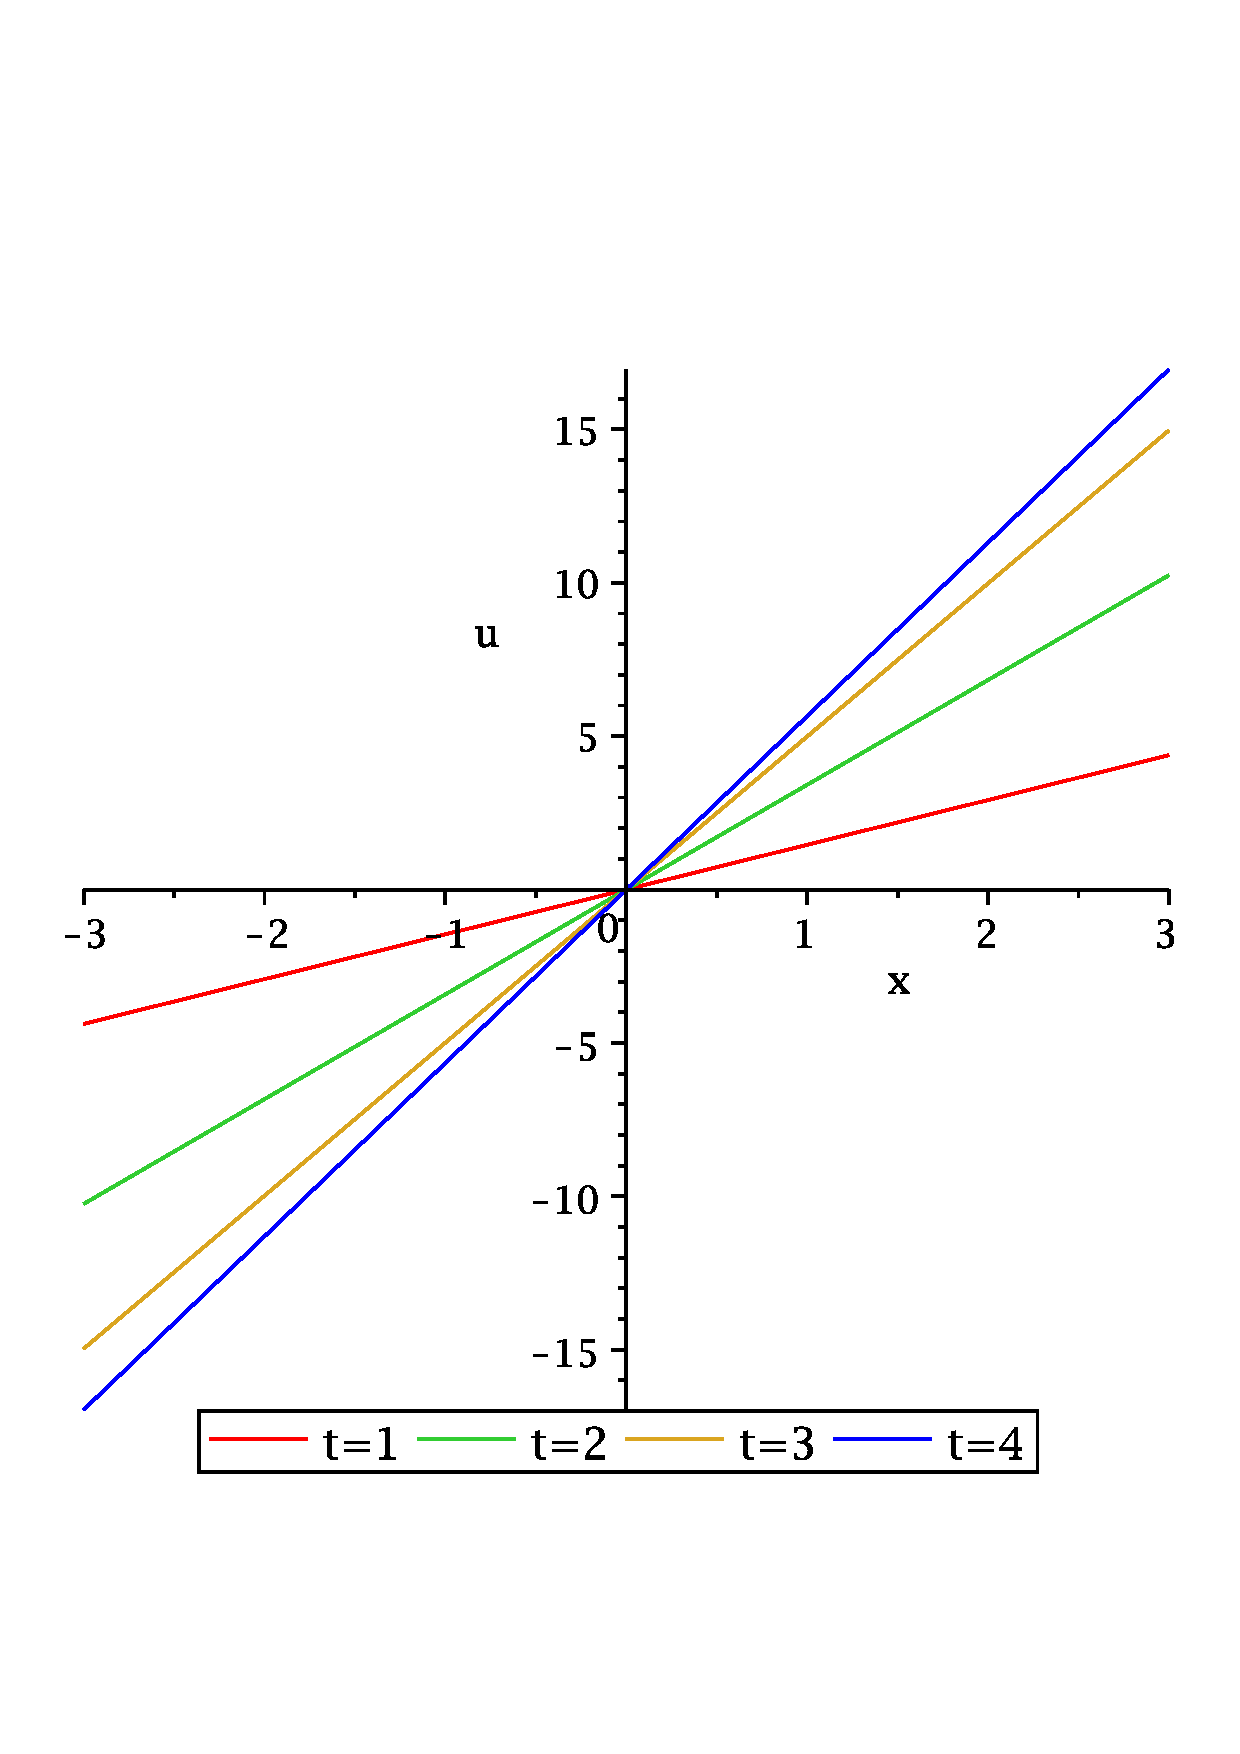
\includegraphics[width=100mm]{ex-1.pdf}
    \caption{The solution $u(x,t)$ for exercise 1 for different values of $t$.}
    \label{fig:ex-1}
\end{figure}


\section*{Exercise 2}
A PDE problem is given by
\begin{gather}
    u_t - ku_{xx} = 0, \quad 0 < x < L, t>0 \nonumber\\
    u(0,t)=at,\quad u(L,t)=0, \quad t > 0 \label{eq:ex2}\\
    u(x, 0) = 0, \quad 0 < x < L \nonumber
\end{gather}
where $a\in\myreal, k>0$ and $L>0$. The solution $u$ for the PDE problem should be found. \par
The PDE is the diffusion equation with inhomogeneous boundary conditions. Therefore the expansion method can be used to find $u$. We look at the Fourier sine series expansion of $u$.
\begin{equation}\label{eq:expansion}
    u(x,t) = \sum_{n=1}^\infty u_n(t)\sin\frac{n\pi x}{L}
\end{equation}
The coefficients $u_n(t)$ can be determined by using equation 5.6.10 in the course textbook (with $j(t)=0, h(t)=at$). The initial condition $u(x,0)=0$ implies that $u_n(0)=0$ and since
\begin{align*}
    u_n(0) &= Ce^{-n^2\pi^2L^{-2}k\cdot0} - 2n\pi L^{-2}k\int_0^0 e^{-n^2\pi^2L^{-2}k(t-s)}(-as)\,ds \\
           &= C
\end{align*}
we get that $C=0$. Using Maple the coefficients are now found as
\begin{align*}
    u_n(t) &= 2n\pi L^{-2}ka\int_0^t e^{-n^2\pi^2L^{-2} k(t-s)}s\,ds \\
    &= \frac{2aL^2}{n^3\pi^3k}(e^{-n^2\pi^2L^{-2}kt} - 1) + \frac{2a}{n\pi}t
\end{align*}
Using these coefficients in (\ref{eq:expansion}) gives the solution to the problem in (\ref{eq:ex2}). To verify the solution the finite sum
\begin{equation*}
    \sum_{n=1}^{100} u_n(t)\sin\frac{n\pi x}{L}
\end{equation*}
is plotted for $a=2, k=1, L=1$ and $t={1,2}$. The plot is shown in figure~\ref{fig:ex2}. The solutions are found to ``approach'' the value $at$ for $x$ ``close'' to 0. The actual value is of cause $u(0, t)=0$ but this is ok since the series isn't bound to converge at the endpoints.

\begin{figure}
    \centering
    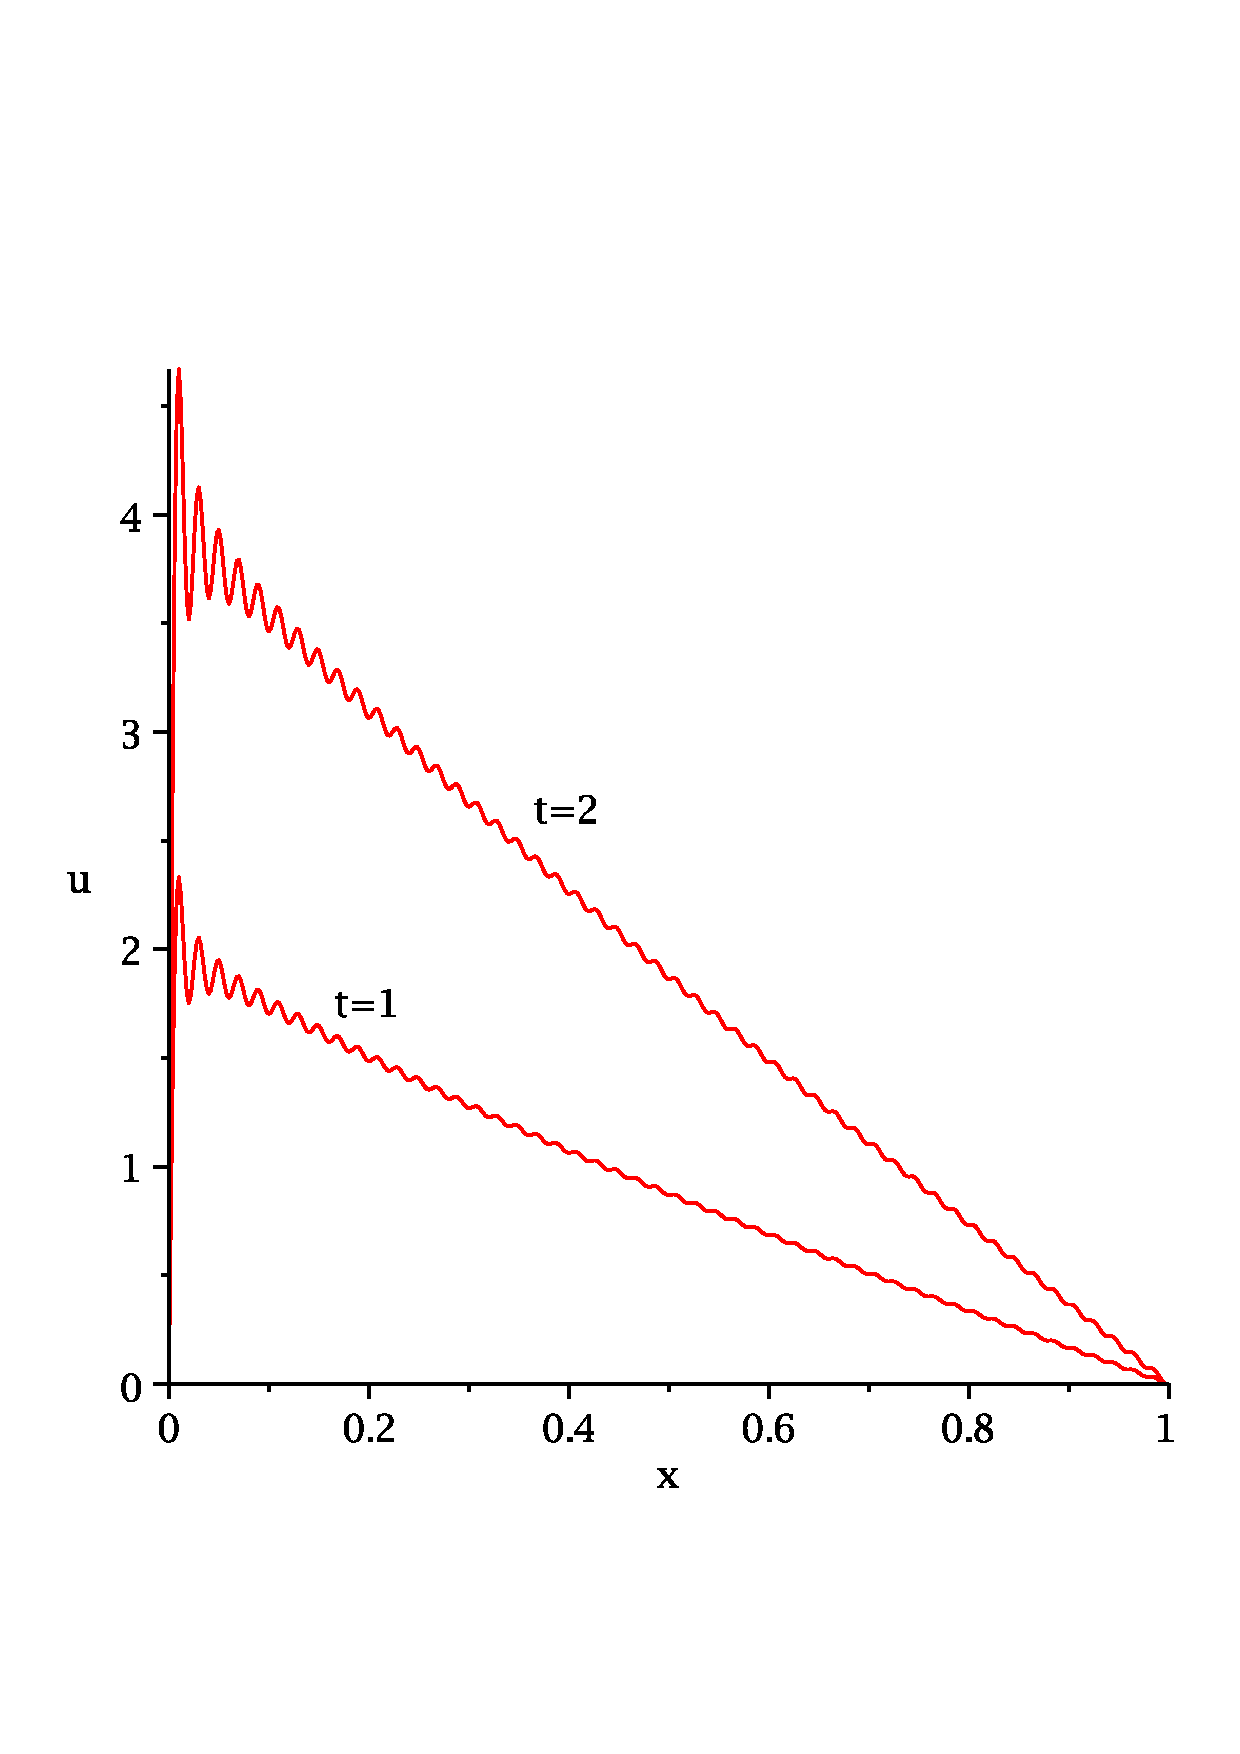
\includegraphics[width=100mm]{ex-2.pdf}
    \caption{The solution for exercise 2 for $t=1,2$. Only the first 100 terms in the solution sum was used and the parameters from the problem statement was chosen as $a=2, k=1$ and $L=1$.}
    \label{fig:ex2}
\end{figure}

\section*{Exercise 3}
A PDE problem for the damped wave equation is given by
\begin{gather}
    u_{tt} + u_t - u_{xx} = 0, \quad 0<x<\pi, t\in\myreal \nonumber\\
    u(x, 0)=0, \quad u_t(x, 0)=\sin(x), \quad 0<x<\pi \label{eq:ex3}\\
    u(0,t)=u(\pi, t)=0,\quad t\in\myreal \nonumber
\end{gather}
A solution for the problem is found by separation of variables. The solution is assumed to be of the form
\begin{equation*}
    u(x,t) = X(x)T(t)
\end{equation*}
Inserted into the PDE this gives
\begin{gather*}
    X(x)T''(t) + X(x)T'(t) - X''(x)T(t) = 0 \myimp \\
    \frac{T''(t) + T'(t)}{T(t)} = \frac{X''(x)}{X(x)} = - \lambda
\end{gather*}
The ODE for $X(x)$ becomes $X''(x) + \lambda X(x) = 0$ which combined with the homogeneous Dirichlet boundary conditions have been solved on page 85 in the course textbook. The eigenvalues and eigenfunctions are therefore given by
\begin{equation*}
    \lambda_n = \left(\frac{n\pi}{l}\right)^2 = n^2, \quad X_n(x) = \sin(nx) \quad (n=1,2,3,\dots)
\end{equation*}
The ODE for $T$ is then
\begin{gather}\label{eq:T-ode}
    T''(t) + T'(t) + n^2T(t) = 0
\end{gather}
The characteristic polynomium is
\begin{gather*}
    s^2 + s + n^2 = 0 \quad\Rightarrow \\
    s = \frac{-1\pm \sqrt{1 - 4n^2}}{2}
\end{gather*}
and since $1-4n^2<0$ for all $n=1,2,3,\dots$
\begin{align*}
    s &= -\frac{1}{2}\pm\sqrt{n^2-\frac{1}{4}}\,\,i
\end{align*}
The general solution for (\ref{eq:T-ode}) is then given by
\begin{align*}
    T(t) = A_n e^{-\frac{t}{2}} \cos\left(\sqrt{n^2-\frac{1}{4}}\,t\right) + B_n e^{-\frac{t}{2}} \sin\left(\sqrt{n^2-\frac{1}{4}}\,t\right)
\end{align*}
From the original problem (\ref{eq:ex3}) we know $u(x,0)=X(x)T(0)=0 \Rightarrow T(0)=A_n=0$ and therefore
\begin{align*}
    u_n(x,t) = B_n e^{-\frac{t}{2}} \sin\left(\sqrt{n^2-\frac{1}{4}}\,t\right) \sin(nx)
\end{align*}
The problem (\ref{eq:ex3}) is linear so any finite sum of solutions is also a solution, so
\begin{align*}
    u(x,t) = \sum_n B_n e^{-\frac{t}{2}} \sin\left(\sqrt{n^2-\frac{1}{4}}\,t\right) \sin(nx)
\end{align*}
The coefficients $B_n$ can be found from the initial condition $u_t(x,0)=\sin(x)$ and since
\begin{align*}
    u_t(x,t) = \sum_n B_n \left(e^{-\frac{t}{2}} \cos\left(\sqrt{n^2-\frac{1}{4}}\,t\right) \sqrt{n^2-\frac{1}{4}} - \frac{1}{2}e^{-\frac{t}{2}} \sin\left(\sqrt{n^2-\frac{1}{4}}\,t\right)\right) \sin(nx)
\end{align*}
we get
\begin{align*}
    u_t(x,0) = \sum_n B_n \sqrt{n^2-\frac{1}{4}} \sin(nx) = \sin(x)
\end{align*}
The coefficients $B_n$ are therefore given by
\begin{equation*}
    B_n = \begin{cases}
        \frac{2}{\sqrt{3}} & n=1 \\
        0 & \text{else}
    \end{cases}
\end{equation*}
which gives the final solution
\begin{equation*}
    u(x, t) = \frac{2}{\sqrt{3}} e^{-\frac{t}{2}}\sin\left(\frac{\sqrt{3}}{2}t\right)\sin(x)
\end{equation*}
In figure~\ref{fig:ex3} the solution is plotted for different values of $t$ and it is seen that the solution match the expected behaviour for a damped wave equation. This behaviour could also be anticipated from the exponentially decreasing function of $t$ in the solution.

\begin{figure}
    \centering
    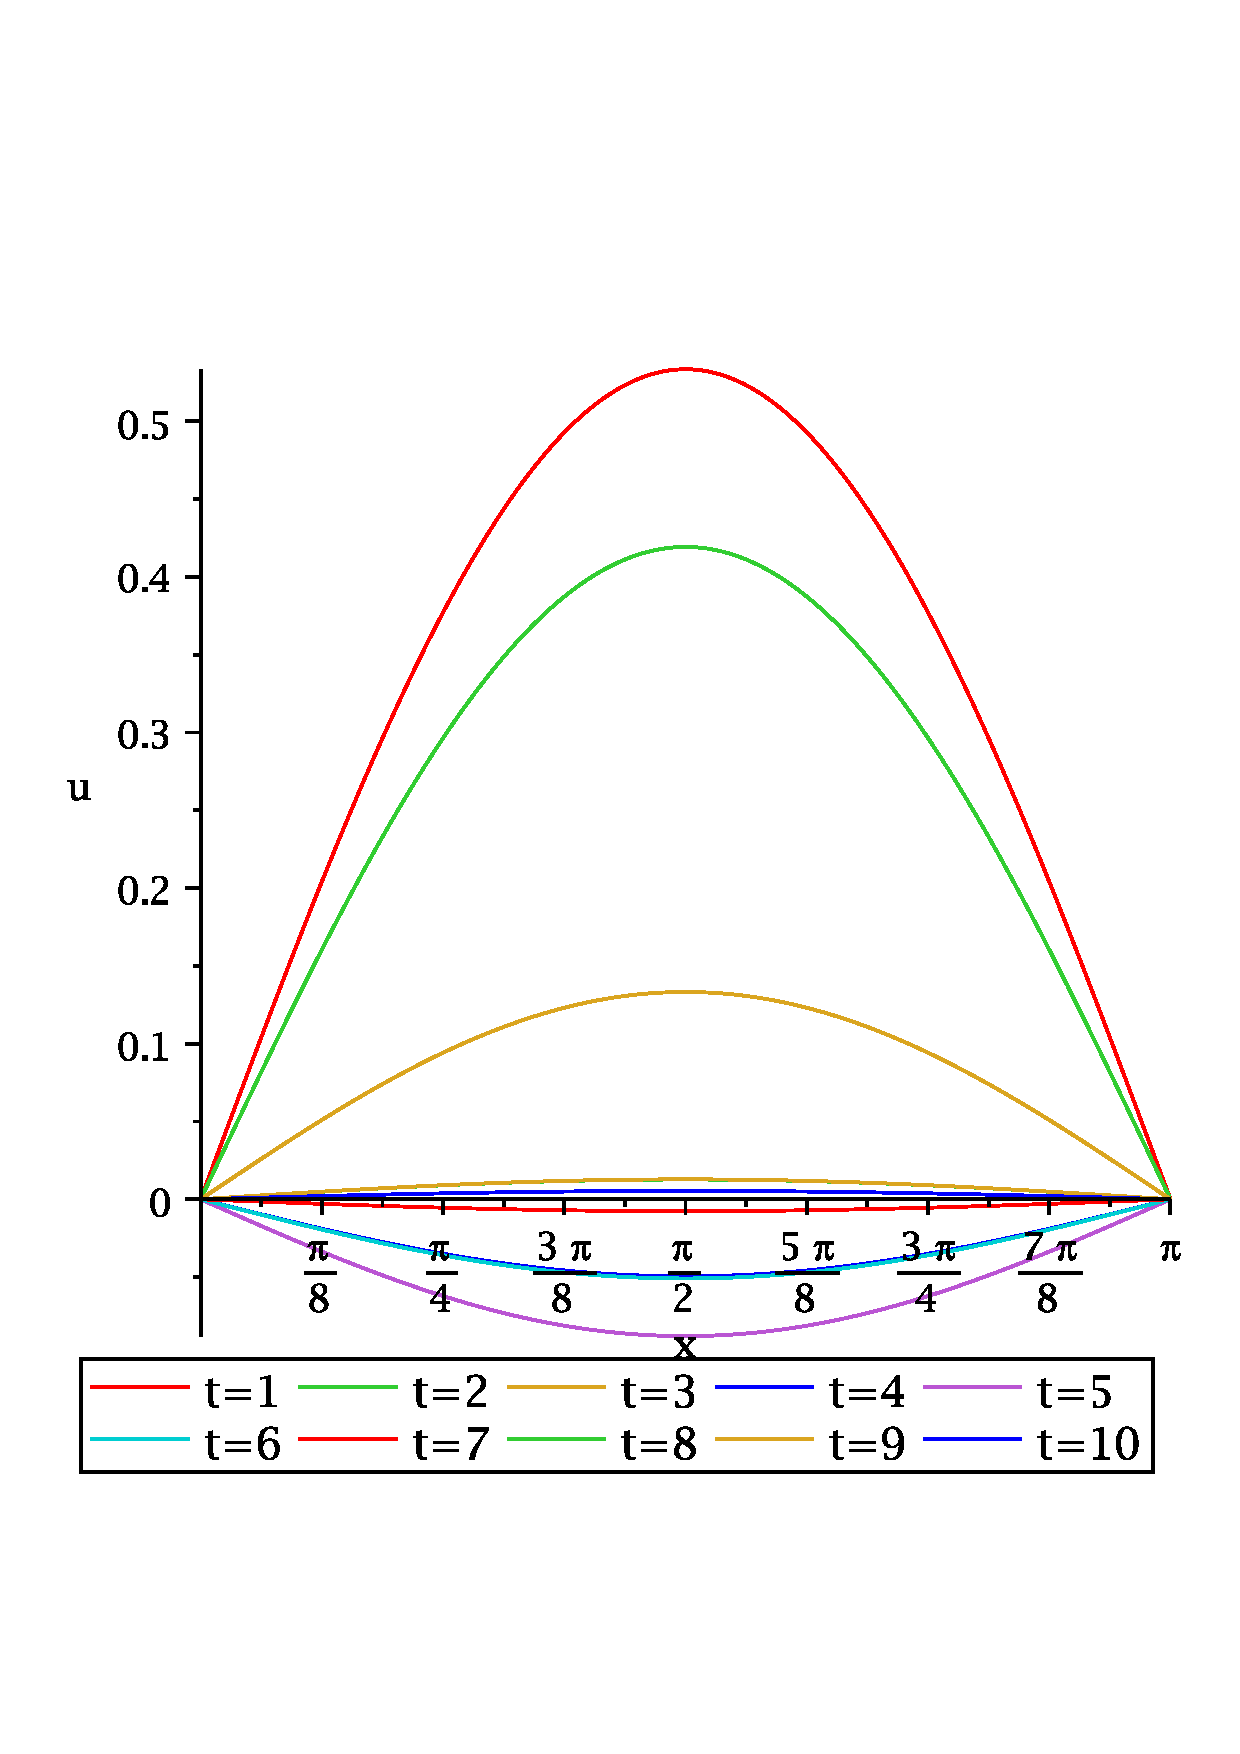
\includegraphics[width=100mm]{ex-3.pdf}
    \caption{The solution $u(x,t)$ for exercise 3 for different values of $t$. The anticipated damped wave behaviour is recognized in the plot.}
    \label{fig:ex3}
\end{figure}

\end{document}
